\section{Durchführung}
\label{sec:Durchführung}
In diesem Versuch werden die gemessene Fließgeschwindigkeit und das Strömungsprofil als Funktion der realen Strömungsgeschwindigkeit und des Dopplerwinkels untersucht. 
Es werden drei verschiedene Leitungen mit Innenradien von $7$, $10$ und $\qty{16}{\milli\metre}$ verwendet. 

\subsection{Vorbereitungsaufgaben}
\label{subsec:Vorbereitung}
Zur Vorbereitung des Versuches sollen die Dopplerwinkel $\alpha_i$ zu verschiedenen Prismenwinkeln $\theta_i$ berechnet werden. Dazu werden der enstprechende Winkel
$\theta$, die Ausbreitungsgeschwindigkeit $c_\text{P} = \qty{2700}{\metre\per\second}$ des Schalles im Prisma und die Ausbreitungsgeschwindigkeit
$c_\text{L} = \qty{1800}{\metre\per\second}$ in der Dopplerphantomflüssigkeit in \autoref{eqn:alpha} eingesetzt, wodurch die Werte
\begin{align*}
    \theta &= \qty{15}{\degree}: \qquad \alpha = \qty{80.04}{\degree} \\
    \theta &= \qty{30}{\degree}: \qquad \alpha = \qty{70.47}{\degree} \\
    \theta &= \qty{60}{\degree}: \qquad \alpha = \qty{54.72}{\degree} \\
\end{align*} 
berechnet werden können.

\subsection{Versuchsaufbau}
\label{subsec:Aufbau}
Zur Durchführung des Versuches wird ein Ultraschall-Doppler-Generator verwendet. Dieser wird im Impuls-Echo-Verfahren mit einer $\qty{2}{\mega\hertz}$ Sonde betrieben.
Untersucht wird ein Rohrkreislauf, in welchem drei Rohre mit unterschiedlichen Durchmessern und zugehörige Prismen verbaut sind. Die Prismen sind an den jeweiligen
Rohrduchmesser angepasst und verfügen über je drei Flächen mit verschiedenem Dopplerwinkel, wobei alle Flächen den gleichen Abstand zur Probe (Flüssigkeit) garantieren.  
Der Aufbau der Prismen ist \autoref{fig:Prisma} zu entnehmen. Es wird eine aus Wasser, Glycerin und
Glasperlen bestehende Dopplerphantomflüssigkeit verwendet, dessen Viskosität $\eta$ und akustischen Eigenschaften auf den Versuchsaufbau abgestimmt sind.
Die Signale des Echoskops werden an einen Rechner übertragen, an welchem sie mithilfe des Programms \textit{FlowView} ausgewertet werden können.

\begin{figure}
    \centering
    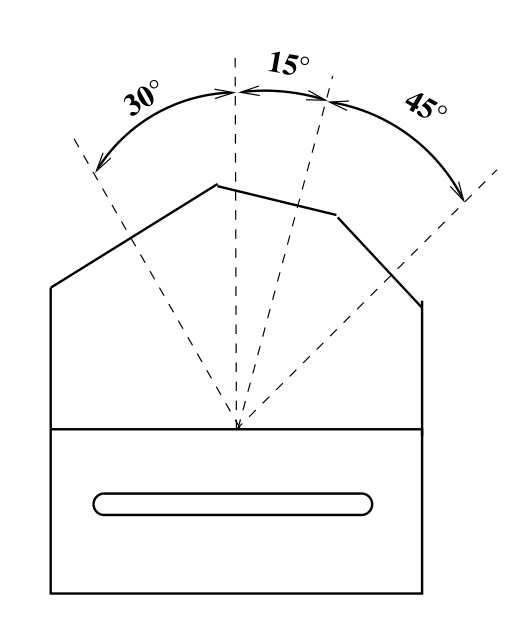
\includegraphics[width=.2\textwidth]{content/Prisma.png}
    \caption{Skizze des Prismas.}
    \label{fig:Prisma}
\end{figure}  

\subsection{Messaufgaben}
\label{subsec:Messaufgaben}
test
